\section{Messaging patterns} \label{section:patterns}
\large \textbf{Apache Kafka}\\
\normalsize
Records on a Kafka topic can be read using Kafka consumer \cite{kafkadesignconsumer}.  Each consumer belongs to one consumer group. A topic on Kafka can be simultaneously consumed by multiple consumer groups, each of which will receive all messages from that topic. 
 
A consumer group can comprise of multiple consumers and each message on the subscribed topic will be delivered to only one of them. The important point is that the messages are not distributed randomly to consumers in the group. Instead, each partition of the topic is assigned to one consumer in the group. At any time, each partition will be assigned and read by only one consumer in the group. 

Each new record appended to a partition is assigned an offset number to be uniquely identified. This offset number is also used by Kafka consumer to indicate its current reading position on the partition. Unlike many traditional messaging systems, Kafka uses pull model to deliver messages to consumer. That means Kafka broker does not keep track of what has been consumed by consumer with acknowledgement and therefore does not actively deliver unread messages to consumer.  It is the responsibility of consumer to provide an offset number indicating its current reading position on every request to pull new batch of messages from that point onward from Kafka. With this approach, the consumer has full control about its reading position. For durability of the consumption status, Kafka supports automatic or manual committing the offset numbers of consumers to internal Kafka topics. Consumer also can maintain its reading position in a different durable storage such as an external relational database.

\textbf{Publish-Subscribe}\\
It is very straightforward to realize the publish-subscribe pattern with the concept of consumer group of Kafka. New subscriber for a topic can be created by creating a new consumer group with only one consumer and all messages on all partitions of that topic will be delivered to this subscriber.

\textbf{Competing consumers}\\

\begin{figure}[h]
	\centering
	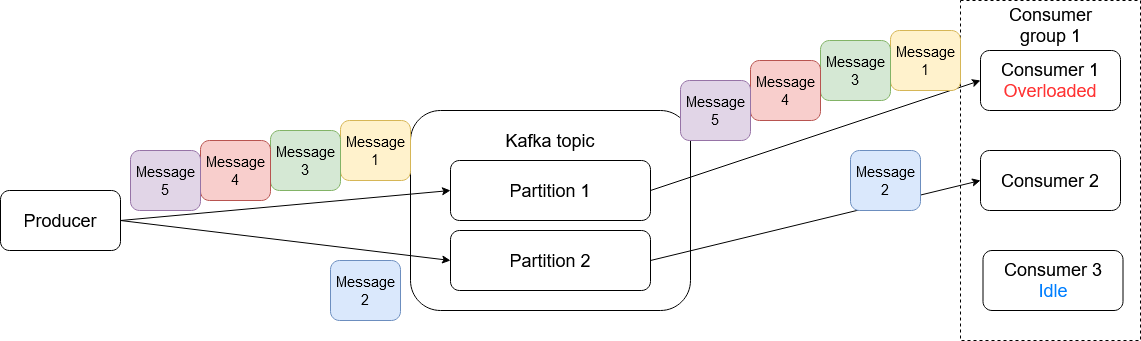
\includegraphics[width=\linewidth,height=5cm]{images/competing-consumers-kafka.png}
	\caption{Competing consumers pattern with Kafka.}
	\label{fig:kafkacompetingconsumer}
\end{figure}
The competing consumers can be realized using consumers within the same group. By adding multiple consumers to one group, they can concurrently consume messages of the subscribed topic and each message will only be read by one consumer. However, since the partition is the unit for parallel consumption in one consumer group, the number of competing consumers will be limited by the number of partitions of the topic. If there are more consumers in the group than partitions, some consumers will be unoccupied. More partitions can allow more parallel consumers. However, if there are too many partitions, this could degrade the performance of the system \cite{kafkapartitionsnum}.

Moreover, if the messages are not evenly distributed across the partitions with some retain more messages than the others, some consumers will have to handle more workload while the others are assigned with empty partitions will remain idle. Therefore, the competing consumers pattern provided by Kafka is quite rigid and cannot be scale freely.

\textbf{Publish-Subscribe + Competing consumers (Consumer group)}\\
Although it can be used as either publish-subscribe or competing consumers pattern for normal messaging scenarios, the concept of consumer group and partition itself is a combination of both these patterns provided by Kafka specifically for the event-driven use cases. By assigning each partition of a topic to a consumer in the consumer group, events of the same type published to the topic can be read and processed in parallel. 

Kafka provides a forwarding mechanism on the producer side to guarantee that events from the same entity will be delivered to the same consumer. Messages in Kafka have the key-value form. If message key is defined, it will be used to create a hash value which will then be used to determine the destination partition of the message. When an identifier is assigned to each event source and used as the key for published events, these events will end up in the same partition on the destination topic. As a result, the consumption of events can be scaled by tuning the number of partitions and consumers in the group while ensuring that each consumer will receive the entire history of events from a specific entity.  

\begin{figure}[h]
	\centering
	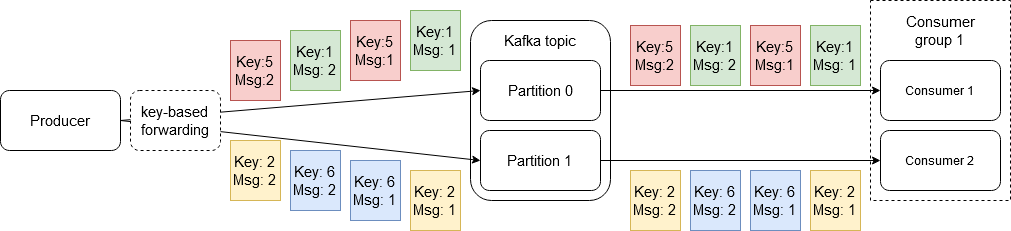
\includegraphics[width=\linewidth,height=4cm]{images/consumer-group-kafka.png}
	\caption{Consumer group pattern with Kafka.}
	\label{fig:kafkaconsumergroup}
\end{figure}


\textbf{Consumer group failover mechanism}\\
Consumers in the group periodically send heartbeats to Kafka to indicate their liveness. Moreover, they must also regularly send new requests for messages from Kafka. If a consumer fails to meet either condition, it is considered to be failed and will be removed by Kafka from the group \cite{kafkaconsumerimplement}. 

In case a consumer fails, its partitions will be reassigned to other consumers in the group automatically. The failover consumer will continue to process messages from the latest reading position of the failed consumer. If this reading position is checkpointed in Kafka, the task of retrieving the consumption status of failed consumer and sending it to the taking-over consumer will be managed transparently by Kafka. On the other hand, if the failed consumer persists its position in an external datastore, Kafka provides the callback \emph{ConsumerRebalanceListener} for consumer to determine when partition rebalancing occurs and retrieve the last reading position on newly assigned partition.

\textbf{Event playback}\\
A Kafka consumer must specify its reading position using offset number in every request to pull new messages from Kafka. Therefore, it is very straightforward to re-consume older records in Kafka by simply using an older offset number for the new consuming request. 

\begin{figure}[h]
	\centering
	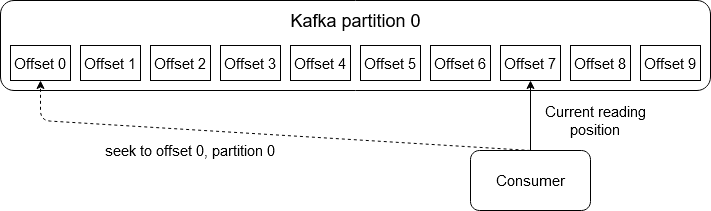
\includegraphics[width=10cm,height=4cm]{images/event-playback-kafka.png}
	\caption{Event playback with Kafka.}
	\label{fig:kafkaeventplayback}
\end{figure}

By default, if a consumer is started with an existing consumer group, its reading position on the assigned partition starts from the latest committed offset number on either Kafka or external datastore, and the position will advance after every request for new messages. However, a Kafka consumer can also reset its reading to an arbitrary position \cite{kafkaconsumerimplement}. This reset operation is done on partition basis. A consumer can only reset the offset of partitions that it is currently assigned to. Next time the consumer pulls more records from this partition, it will start from the reset offset position.

\large \textbf{Apache Pulsar}\\
\normalsize
There are two ways to consume message from Pulsar, namely, using Pulsar consumer and Pulsar reader.

The consumption of messages with Pulsar consumer is quite similar to traditional messaging system. Pulsar uses a combination of push and pull models to deliver messages to consumer \cite{pulsarbinaryprotocol}. Acknowledgement must be sent back to Pulsar broker upon successful processing of a message. The broker will keep track of the consumption status of consumers and will send unacknowledged messages to a queue on the consumer side when it receives permission from the consumer. Messages on this queue is dequeued and consumed gradually by the application. Once the queue is halved, Pulsar consumer sends a new request for new messages to be pushed to the queue again. Moreover, Pulsar broker also uses the acknowledgements to mark messages as being able to be deleted.

Consumers subscribe to a topic by creating a subscription \cite{pulsarconceptmessaging}. Multiple consumers can be grouped together with the same subscription to consume messages on the topic together. There are four different subscription modes, namely, Exclusive, Failover, Shared and Key\_Shared each of which is relevant to a different messaging pattern supported by Pulsar. However, with the current release of Pulsar, the Key\_Shared subscription mode is still unstable \cite{pulsarkaysharedunstable}. Therefore, this mode will not be considered further in the thesis.

On the other hand, the Pulsar reader is internally a Pulsar consumer with special configurations \cite{pulsarconceptclients}. The Pulsar broker does not monitor the consumption status of reader and does not require acknowledgement of messages. Therefore, Pulsar broker does not control which messages to be delivered to reader. On starting up, the reader must define a specific starting position by giving the ID of the first message to be read and only messages from that point onward will be delivered to the reader. This reader is designed to give users more control over which messages to be read from Pulsar and is quite similar to Kafka consumer. If the reader needs durable consumption status, it has to maintain its own current reading position in a durable storage and manually retrieve that on every startup. Pulsar does not support auto-checkpointing reader position natively on Pulsar as in Kafka. 

However, there is no possibility like subscription to group multiple readers together. Each reader connects directly to a topic and starts consuming all messages individually. Therefore, it is not possible to realize messaging patterns of shared consumption such as competing consumers and consumer group with Pulsar reader. Moreover, at the moment with Pulsar 2.7.0, a Pulsar reader can only read from non-partitioned topics.

\textbf{Publish-Subscribe}\\
Pulsar provides the Publish-Subscribe pattern with the Exclusive subscription mode of consumer. In this mode, at any time, only one consumer is allowed in the subscription, other consumers which join the subscription later will be rejected. All messages on the subscribed topic will be delivered to the single consumer in the subscription. Different subscribers can create a new exclusive subscription to the topic with different subscription names.

The publish-subscribe pattern can also be realized with the Pulsar reader. Multiple readers on a non-partitioned topic can simply be started and every message on the topic will be delivered to all of them. 

\textbf{Competing consumers}\\
This pattern is realized on Pulsar with the Shared subscription mode. Multiple consumers can be grouped together using this mode. Messages will be distributed to the consumers in a round-robin fashion and each message will be delivered to only one consumer in the group.

\textbf{Publish-Subscribe + Competing consumers (Consumer group)}\\
Like Kafka, messages on Pulsar have the key-value form. If a message is created without a key, it will be delivered to a random partition of the topic. But if a key value is assigned, its hashed value will be used to determine the target partition for the message on the topic. On Pulsar, to enable the combination of Publish-Subscribe and Competing consumers, on the producer side, key values must be assigned to all generated events. They will be used as identifiers for events from the same source and help deliver them to only one consumer.

On consumer side, Failover subscription mode can be used to realize this pattern. In this mode, multiple consumers can be grouped together into the same subscription. Each partition of the subscribed topic will be assigned to only one consumer in the group. Only if a consumer fails, its partitions will be taken over by another consumer in the subscription. By adding key to each event on the producer side, it is ensured that events of the same entity will be on the same partition and therefore a consumer in the subscription will receive all of them. This is similar to the consumer group in Kafka and it requires the topic to be partitioned to enable this parallel consumption. The level of parallelism is also limited by the number of partitions of the topic. 

\begin{figure}[h]
	\centering
	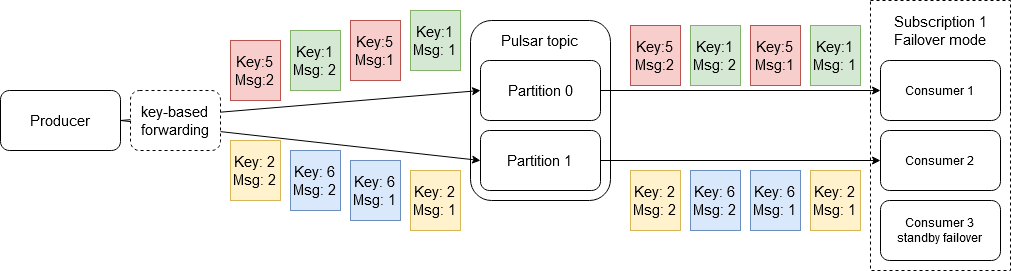
\includegraphics[width=\linewidth,height=4cm]{images/consumer-group-pulsar.png}
	\caption{Consumer group pattern with Pulsar.}
	\label{fig:pulsarconsumergroup}
\end{figure}

\textbf{Consumer group failover mechanism}\\
In Failover mode, each partition of the topic is assigned to one consumer in the subscription. Pulsar broker automatically monitors the connection to every consumer. 

If a consumer disconnects, its partitions will be assigned to other consumers automatically by Pulsar. Moreover, because Pulsar broker keeps track of the consumption statuses of all consumers with acknowledgement, it will know which messages have not been read by the failed consumer and continue to deliver them to the failover consumer.

\textbf{Event playback}\\
For Apache Pulsar, event playback is possible with both Consumer and Reader API.

Pulsar consumer must acknowledge the consumption of each message. It is the responsibility of the broker to decide which messages will be delivered based on the acknowledgements received from the consumer. By default, if a consumer is started with an existing subscription, the reading will automatically be started from the earliest unacknowledged message onward. Nevertheless, it is also possible to reset the consuming position of the subscription with Consumer API \cite{pulsarconsumerapi}. User can reset reading position to a message with a specific message ID. The message ID must be known beforehand. It is also possible to reset the reading position of the subscription to message published at the time equal or greater than a specified timestamp. 

With Pulsar reader, a starting position of messages to be read from the topic must be specified every time it is started. As a result, the reader has the flexibility to jump to arbitrary positions and replay events on the topic whenever needed \cite{pulsarreaderapi}. The starting position can be defined by providing a message ID. User can also specify a rollback duration to rewind the reading position to a specific time point. The times semantics of both consumer and reader is when the messages were published and were automatically assigned by the Pulsar producer.
\begin{figure}[h]
	\centering
	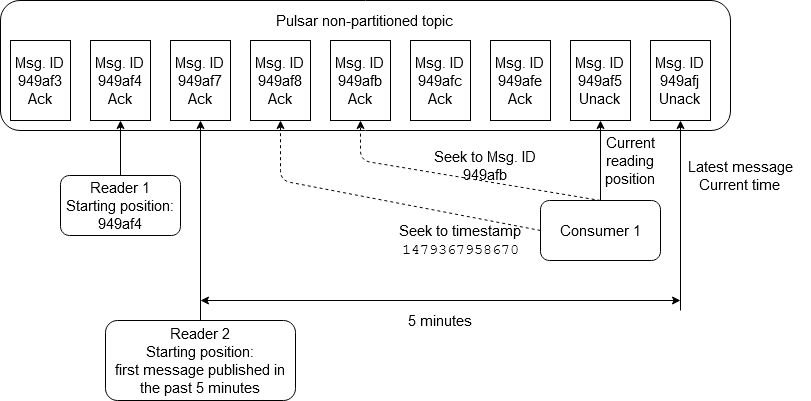
\includegraphics[width=\linewidth,height=5cm]{images/event-playback-pulsar.png}
	\caption{Event playback with Pulsar.}
	\label{fig:pulsareventplayback}
\end{figure}

\large \textbf{NATS Streaming}\\
\normalsize
With NATS Streaming client API, a consumer must create a subscription to a channel to be able to start consuming messages \cite{natsconceptchannels}. NATS Streaming provide two subscription modes. The first is normal mode which means there is only one consumer per subscription, and it will receive all messages on the channel. The second mode is queue mode where a subscription has multiple competing consumers which will read the same topic and each message will be read by only one consumer. 

NATS streaming uses push model to deliver messages to subscriber. That means the server controls which messages to be sent to consumer. The server keeps up with the current consumption status of each consumer by receiving acknowledgements. NATS server actively pushes next unacknowledged messages to the consumer and expects that the receiving application is available to process these messages right away. Consumer must acknowledge with server about the successful consumption of every message within a predefined time window. Otherwise, unacknowledged messages will be redelivered to subscriber after timeout. 
 
By default, NATS server only retains the consumption status of a consumer during the connection session. When being disconnect, the current reading position of the consumer will not be remembered by the server. In this case, if the consumer wants to resume its consumption from the previous session, it must maintain its own reading position in an external storage and provides it as the starting position to read when reconnecting to the server. 

To have a durable consumption status on the server which will be automatically resumed when the consumer reconnects, the subscription must be strictly configured to be durable. When a subscriber starts consuming messages using an existing durable subscription, it will resume its consumption of the unacknowledged messages from the previous connection session.

\textbf{Publish-Subscribe}\\
In NATS Streaming, a new subscriber to a channel can be set up by simply starting a consumer in normal mode with a new client ID and all messages on that channel will be delivered to this new consumer. 

\textbf{Competing consumers}\\
Competing consumers for a topic can be grouped together into a subscription with queue mode. NATS Streaming will deliver messages to consumers in the group randomly and each message will be sent to only one consumer. The number of consumers in a queue group can be scaled freely.

\textbf{Publish-Subscribe + Competing consumers (Consumer group)}\\
NATS Streaming offers no combination of Publish-Subscribe and Competing consumers patterns. The subscriber in Publish-Subscribe pattern is not scalable. On the other hand, with the competing consumers pattern, it is not guaranteed that all events from one source will be delivered to the same consumer because of the random distribution of message in the group. If parallel consumption of events is needed, it must be self-implemented by user on the channel level. In this case, all the task of partitioning events of the same type into multiple channels, forwarding events from the same source to the same channel and assigning each channel to one subscriber will have to be done manually.

\textbf{Consumer group failover mechanism}\\
Since the consumer group pattern is not supported by NATS Streaming, there is also no failover mechanism.

\textbf{Event playback}\\
Event playback with NATS Streaming is very straightforward. When creating a subscriber to a NATS channel, user has the ability to choose different starting positions for the subscription \cite{natsdevelopingreceivemessage}. Consumer can start consuming messages from a specific sequence number on the channel, from a specific starting time or from a rewind duration. The time semantics here is when a message is stored on the NATS server and is managed by the server.
\begin{figure}[h]
	\centering
	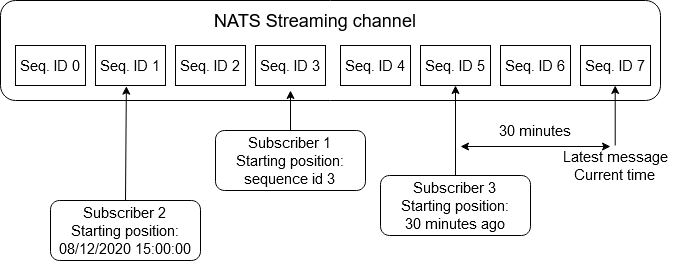
\includegraphics[width=\linewidth,height=5cm]{images/event-playback-nats.png}
	\caption{Event playback with NATS Streaming.}
	\label{fig:natseventplayback}
\end{figure}

By default, the subscription on NATS Streaming is not durable. Thus, when a subscriber disconnects to the server, its current reading position will be lost. As a result, user can choose a different starting position every time the subscriber is restarted and can freely jump to different messages on the channel. In case of durable subscription, the current reading position of the subscriber is kept track by the server. Therefore, to replay events, subscriber must first unsubscribe the durable subscription before it can specify a new reading position using the same subscription name.







